\documentclass[12pt]{article}

% 基础宏包
\usepackage{graphicx}  % 插入图片
\usepackage[english]{babel}  % 英语语言支持
% \usepackage[UTF8]{ctex}  % 如果不需要中文，可以注释掉这一行

% 数学宏包
\usepackage{amsmath}  % 数学排版增强
\usepackage{amsfonts} % 数学字体

% 图表相关
\usepackage{float}    % 浮动体控制 [H] 选项
\usepackage{tikz}     % 绘图
\usepackage{pgfplots} % 函数绘图
\pgfplotsset{compat=1.18} % 设置pgfplots兼容性

% 页面设置
\usepackage{geometry}
\geometry{
  a4paper,
  left=2cm,
  right=2cm,
  top=2cm,
  bottom=2cm
}

% 版式设置
\usepackage{fancyhdr}    % 页眉页脚
\usepackage{lastpage}    % 最后一页引用
\usepackage{multicol}    % 多栏排版
\usepackage{tabularx}    % 表格增强

% 文本修饰
\usepackage{ulem}        % 下划线等
\usepackage{enumitem}    % 列表样式
\usepackage{titlesec}    % 标题样式
\usepackage[export]{adjustbox} % 图片对齐

% 颜色
\usepackage{color}       % 颜色支持

\linespread{1.5}         % 1.5倍行距

\title{Lab 2}
\author{Emilien Zhang}
\date{31 March 2026}

\begin{document}

\maketitle

\section*{Problem 1}

\begin{figure}[H]
  \centering
  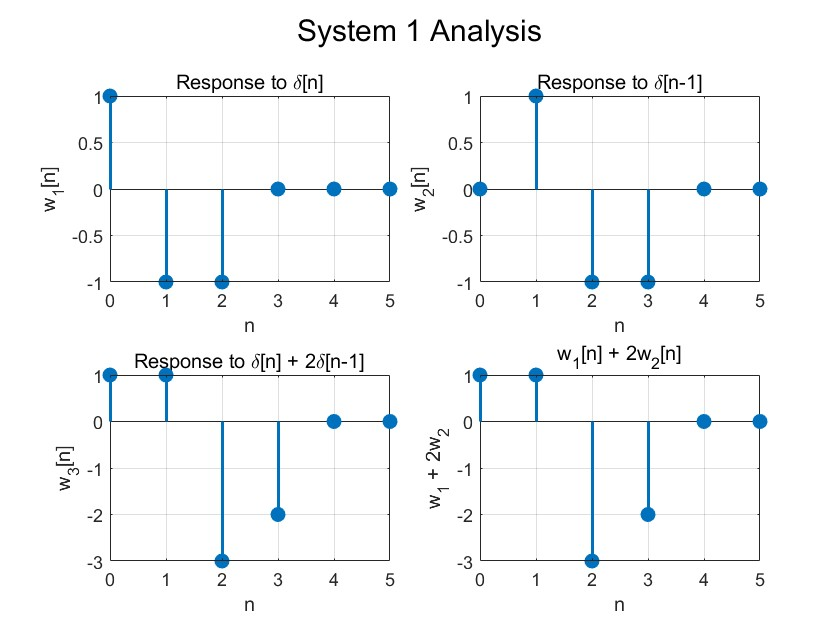
\includegraphics[width=1.0\textwidth]{1.1.jpg}
  \caption{Figure for problem 1}
  \label{fig1}
\end{figure}

From the MATLAB computation, we observe that 

\(w_3[n] = w_1[n] + 2w_2[n] , y_3[n] \neq y_1[n] + 2y_2[n] , z_3[n] = z_1[n] + 2z_2[n]\).



\subsection*{1 Linearity}

A system is linear if it satisfies the superposition principle:
\[
T\{a x_1[n] + b x_2[n]\} = a T\{x_1[n]\} + b T\{x_2[n]\}
\]
for any constants \(a, b\) and any inputs \(x_1[n], x_2[n]\).

\subsubsection*{System 1}

For any \(a, b\) and inputs \(x_1[n], x_2[n]\):
\begin{align}
T(ax_1 + bx_2) &= (ax_1[n] + bx_2[n]) - (ax_1[n-1] + bx_2[n-1]) - (ax_1[n-2] + bx_2[n-2]) \\
&= a[x_1[n] - x_1[n-1] - x_1[n-2]] + b[x_2[n] - x_2[n-1] - x_2[n-2]] \\
&= aT(x_1) + bT(x_2)
\end{align}
Therefore, the system is linear.

\subsubsection*{System 2}

Consider \(x_1[n] = \delta[n]\) and \(x_2[n] = \delta[n-1]\), with \(a = 1\), \(b = 2\).

Left-hand side (LHS):
\[
T(\delta[n] + 2\delta[n-1]) = \cos(\delta[n] + 2\delta[n-1])
\]
At \(n = 0\):
\[
y_3[0] = \cos(1 + 0) = \cos(1) \approx 0.5403
\]

Right-hand side (RHS):
\[
T(\delta[n]) + 2T(\delta[n-1]) = \cos(\delta[n]) + 2\cos(\delta[n-1])
\]
At \(n = 0\):
\[
y_1[0] + 2y_2[0] = \cos(1) + 2\cos(0) = 0.5403 + 2 = 2.5403
\]

Since \(0.5403 \neq 2.5403\), the superposition principle fails. Therefore, System 2 is nonlinear.

\subsubsection*{System 3}

 For any constants \(a, b\) and inputs \(x_1[n], x_2[n]\):
\begin{align}
T(ax_1 + bx_2) &= n \cdot (ax_1[n] + bx_2[n]) \\
&= a(n \cdot x_1[n]) + b(n \cdot x_2[n]) \\
&= aT(x_1) + bT(x_2)
\end{align}
This satisfies both homogeneity and additivity. Therefore, System 3 is linear.
\subsection*{2 Time-Invariance}


A system is time-invariant if a time shift in the input results in an identical time shift in the output:
\[
\text{If } y[n] = T\{x[n]\}, \text{ then } y[n - n_0] = T\{x[n - n_0]\} \text{ for any integer } n_0
\]

Only System 3 is time-variant, because the coefficient \(n\) explicitly depends on time.

\subsection*{3 Summary}
\begin{table}[H]
\centering
\caption{Summary of Results}
\begin{tabular}{|c|c|c|c|}
\hline
\textbf{System} & \textbf{Input-Output Relation} & \textbf{Linearity} & \textbf{Time-Invariance} \\
\hline
1 & $w[n] = x[n] - x[n-1] - x[n-2]$ & \textcolor{blue}{Linear} & \textcolor{blue}{Time-Invariant} \\
2 & $y[n] = \cos(x[n])$ & \textcolor{red}{Non-Linear} & \textcolor{blue}{Time-Invariant} \\
3 & $z[n] = n \cdot x[n]$ & \textcolor{blue}{Linear} & \textcolor{red}{Time-Variant} \\
\hline
\end{tabular}
\end{table}

\section*{Problem 2}

\subsection*{1 Unit Step/Impulse Response}

The unit step response and unit impulse response of the causal LTI system described by
\[
\frac{dy(t)}{dt} + 3y(t) = x(t)
\]
are:

\[
\boxed{s(t) = \frac{1}{3}\left(1 - e^{-3t}\right)u(t)}
\]

\[
\boxed{h(t) = e^{-3t}u(t)}
\]

The impulse response is the derivative of the step response:
\[
h(t) = \frac{ds(t)}{dt} = e^{-3t}u(t)
\]

\begin{figure}[H]
  \centering
  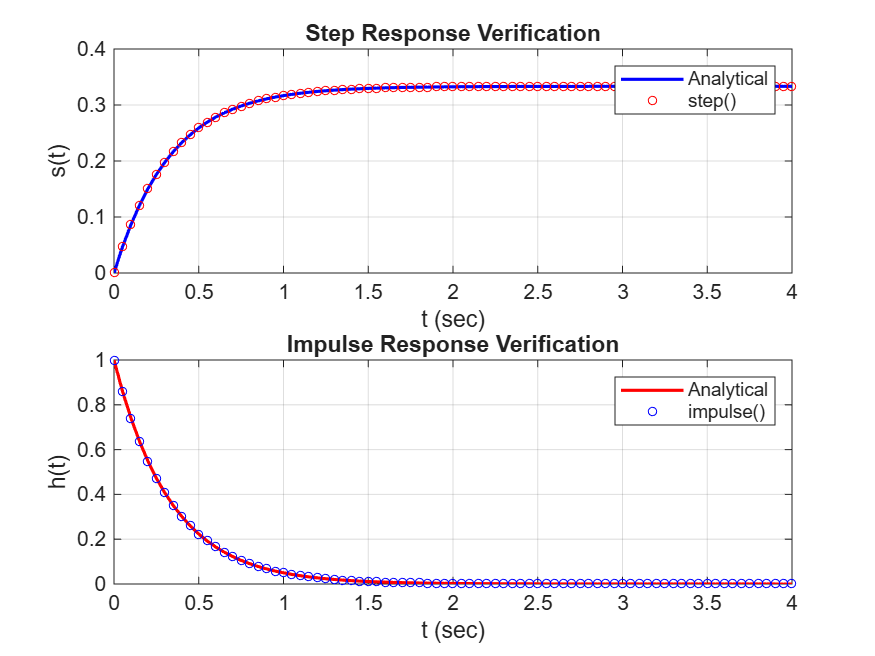
\includegraphics[width=1.0\textwidth]{2.2_2.png}

  \caption{Unit step and unit impulse responses}
  \label{fig2}
\end{figure}

\subsection*{2 Pulse Response \(h^\Delta(t)\)}

The pulse \(\delta^\Delta(t)\) is defined as:
\[
\delta^\Delta(t) = 
\begin{cases}
\frac{1}{\Delta}, & 0 \leq t < \Delta \\
0, & \text{otherwise}
\end{cases}
\]
with unit area \(\int_{-\infty}^{\infty} \delta^\Delta(t) dt = 1\).

We can derive that as \(\Delta\) decreases, \(h^\Delta(t)\) approaches \(h(t)\). In the limit:
\[
\lim_{\Delta \to 0} h^\Delta(t) = h(t)
\]

\begin{figure}[H]
  \centering
  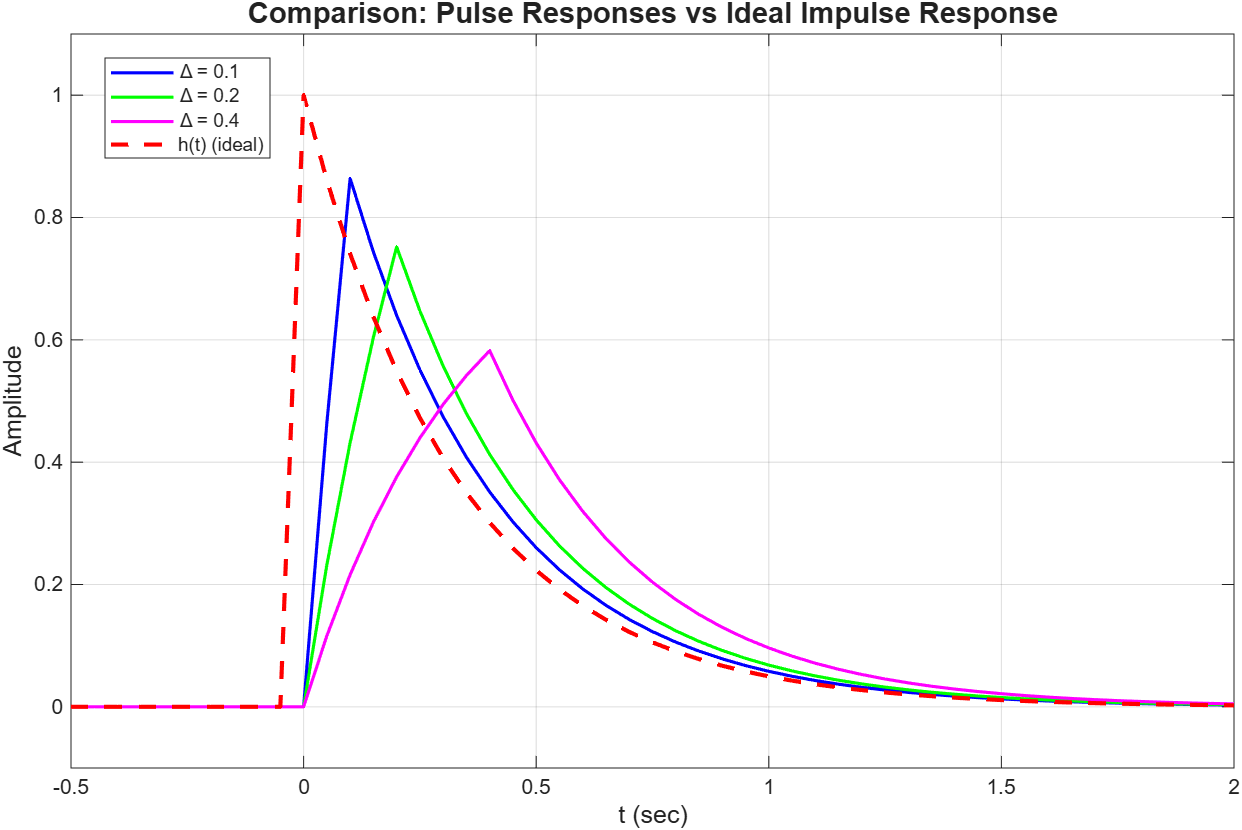
\includegraphics[width=1.0\textwidth]{2.2_15.png}
  \caption{Pulse response}
  \label{fig3}
  \end{figure}


The pulse \(D^\Delta(t)\) is defined as:
\[
D^\Delta(t) = 
\begin{cases}
1, & 0 \leq t < \Delta \\
0, & \text{otherwise}
\end{cases}
\]
with area \(\int_{-\infty}^{\infty} D^\Delta(t) dt = \Delta\).

Since \(\delta^\Delta(t) = \frac{1}{\Delta} D^\Delta(t)\) and the system is linear:
\[
T\{D^\Delta(t)\} = \Delta \cdot T\{\delta^\Delta(t)\} \to \Delta \cdot h(t)
\]


\begin{figure}[H]
  \centering
  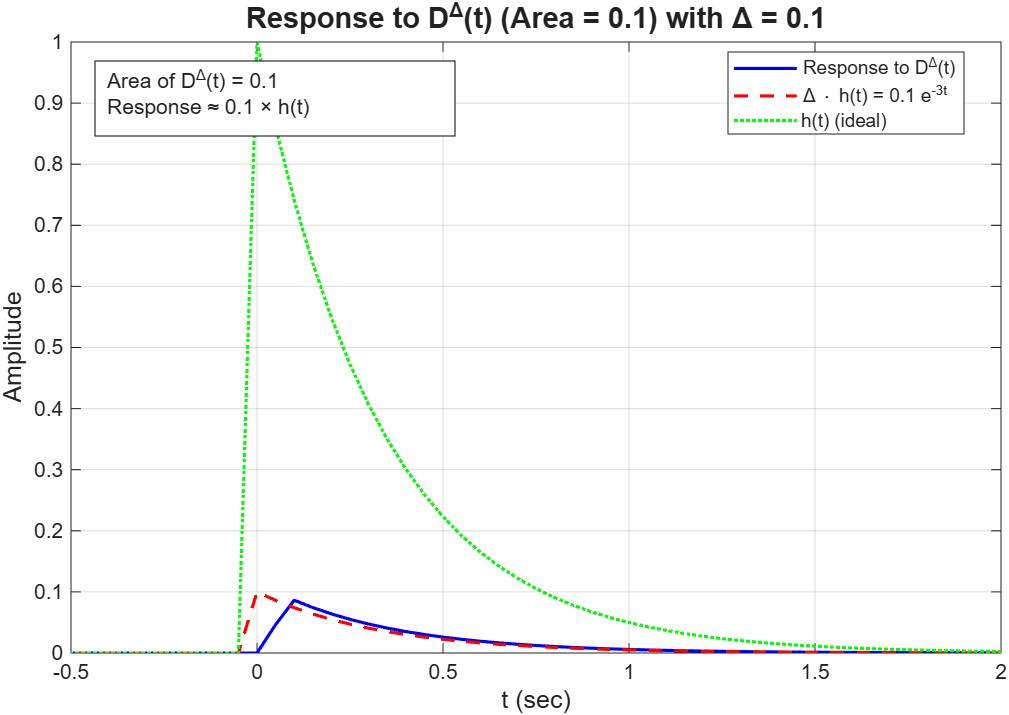
\includegraphics[width=0.5\textwidth]{2.2_17.png}
  \caption{Pulse response when \(\Delta = 0.1\)}
  \label{fig4}
  \end{figure}

  \begin{figure}[H]
  \centering
  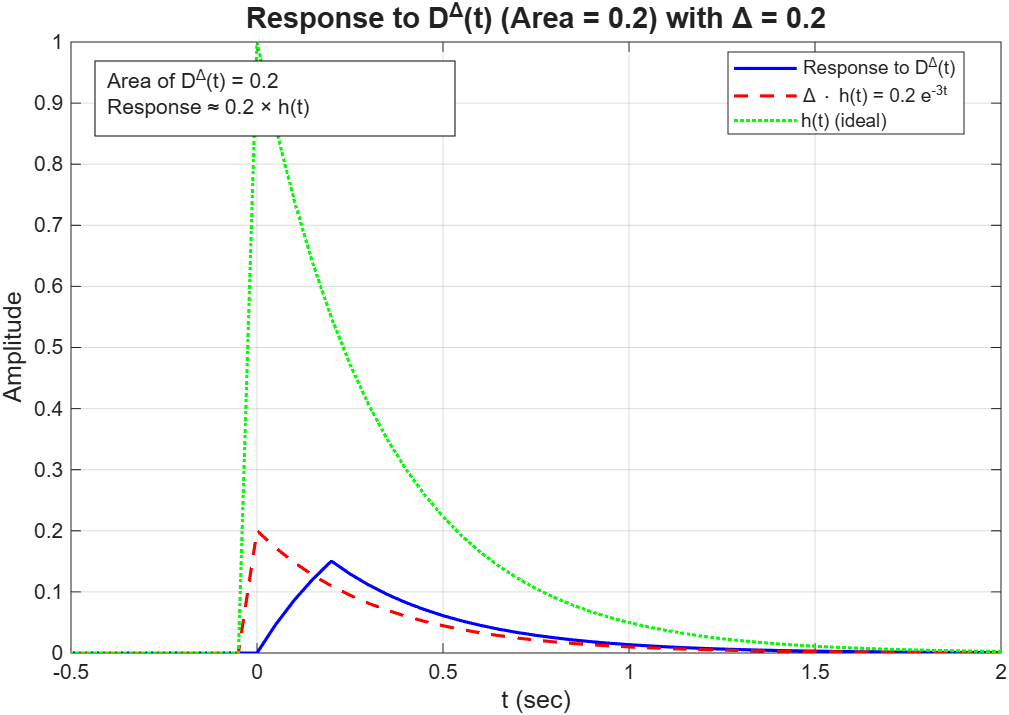
\includegraphics[width=0.5\textwidth]{2.2_18.png}
  \caption{Pulse response when \(\Delta = 0.2\)}
  \label{fig5}
  \end{figure}
  \begin{figure}[H]
  \centering
  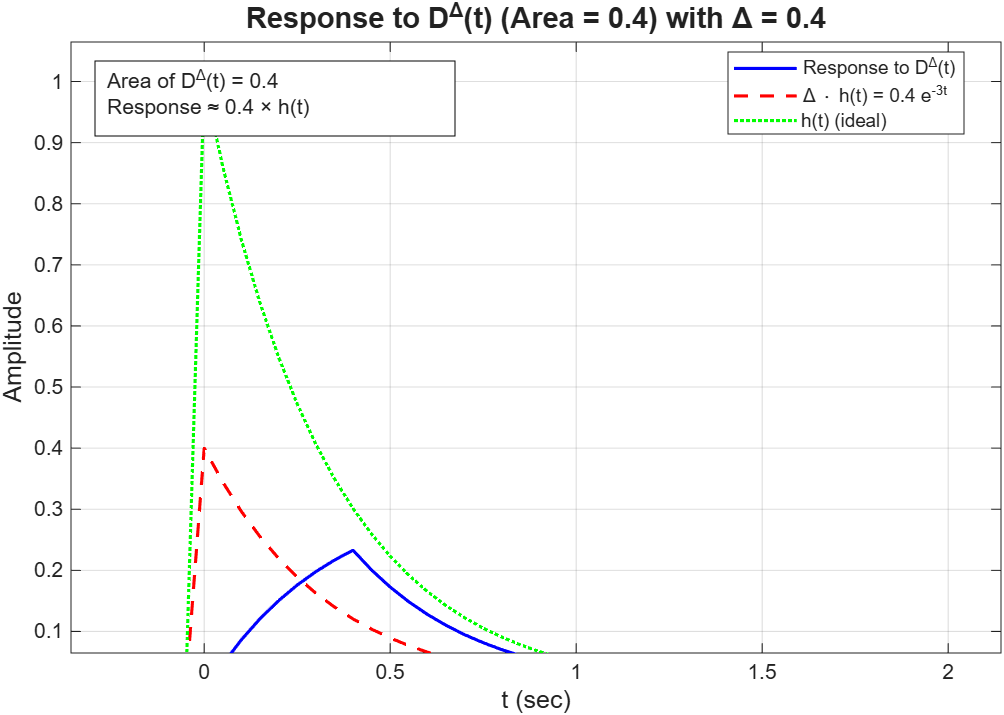
\includegraphics[width=0.5\textwidth]{2.2_19.png}
  \caption{Pulse response when \(\Delta = 0.4\)}
  \label{fig6}
  \end{figure}

We can derive that unit area is necessary because:
\begin{itemize}
    \item The Dirac delta \(\delta(t)\) is defined to have unit area.
    \item To approximate \(\delta(t)\), the pulse must also have unit area.
    \item If the pulse has area \(A \neq 1\), the response will be \(A \cdot h(t)\) instead of \(h(t)\).
\end{itemize}

\subsection*{3 \(d_a(t) = a e^{-at} u(t)\)}


The area of \(d_a(t)\) is:

\[
\int_{-\infty}^{\infty} d_a(t) \, dt = \int_0^{\infty} a e^{-at} \, dt = a \cdot \left[ \frac{e^{-at}}{-a} \right]_0^{\infty} = a \cdot \left( 0 - \left(-\frac{1}{a}\right) \right) = 1
\]

\[
\boxed{\text{Area of } d_a(t) = 1 \quad \text{for all } a > 0}
\]

Thus, \(d_a(t)\) has unit area regardless of the value of \(a\).


As \(a \to \infty\):
\begin{itemize}
    \item The function \(d_a(t) = a e^{-at} u(t)\) becomes increasingly narrow
    \item The peak at \(t = 0\) increases: \(d_a(0) = a\)
    \item The width decreases: most energy is in \([0, 4/a]\)
    \item The area remains constant at 1
\end{itemize}

Therefore:
\[
\lim_{a \to \infty} d_a(t) = \delta(t)
\]

\begin{figure}[H]
  \centering
  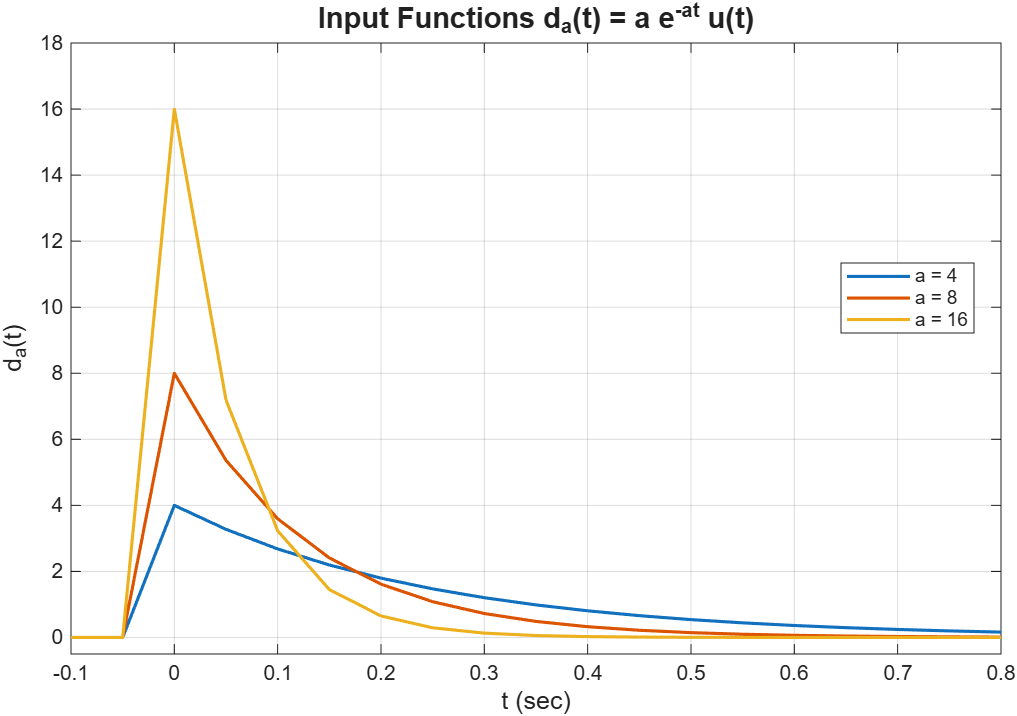
\includegraphics[width=1\textwidth]{2.2_21.png}
  \caption{input function \(d_a(t)\)}
  \label{fig7}
  \end{figure}



The LTI system is described by:
\[
\frac{dy(t)}{dt} + 3y(t) = x(t)
\]
with impulse response \(h(t) = e^{-3t}u(t)\).

Due to linearity and time-invariance, the response to \(d_a(t)\) is the convolution:
\[
y_a(t) = (d_a * h)(t) = \int_0^t a e^{-a\tau} \cdot e^{-3(t-\tau)} \, d\tau = e^{-3t} \int_0^t a e^{-(a-3)\tau} \, d\tau
\]

For large \(a\) (\(a \gg 3\)), \(d_a(t)\) approximates \(\delta(t)\), so:
\[
y_a(t) \approx h(t)
\]





\begin{figure}[H]
  \centering
  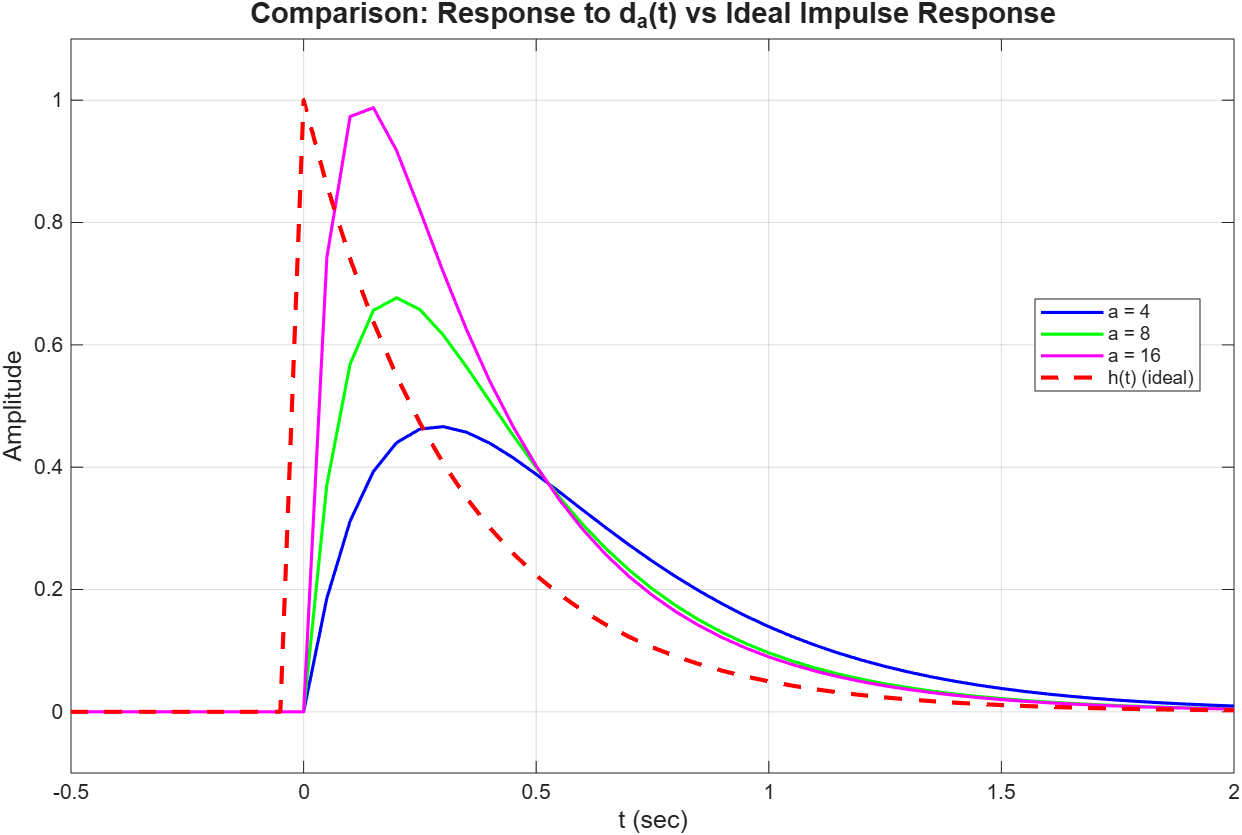
\includegraphics[width=1\textwidth]{2.2_20.png}
  \caption{response to \(d_a(t)\) for \(a = 4, 8, 16\)}
  \label{fig8}
  \end{figure}



As \(a\) increases:
\begin{itemize}
    \item The input \(d_a(t)\) becomes narrower and taller
    \item The response \(y_a(t)\) approaches the ideal impulse response \(h(t) = e^{-3t}u(t)\)
    \item For \(a = 16\), the response is practically identical to \(h(t)\)
\end{itemize}


For sufficiently large \(a\) (\(a \gg 3\)), the response to \(d_a(t)\) is virtually indistinguishable from the true impulse response \(h(t)\). This is because:
\begin{enumerate}
    \item \(d_a(t)\) has unit area for all \(a\)
    \item As \(a \to \infty\), \(d_a(t) \to \delta(t)\)
    \item For an LTI system, \(T\{\delta(t)\} = h(t)\)
\end{enumerate}

\section*{Problem 3}


The echo system is described by:
\[
y[n] = x[n] + \alpha x[n - N]
\]

For an impulse input \(x[n] = \delta[n]\), the output is the impulse response:
\[
h_e[n] = \delta[n] + \alpha \delta[n - N]
\]

With the given parameters \(N = 1000\) and \(\alpha = 0.5\):
\[
\boxed{h_e[n] = \delta[n] + 0.5\,\delta[n - 1000]}
\]

The impulse response has non-zero values only at:
\begin{itemize}
    \item \(n = 0\): \(h_e[0] = 1\) (direct path)
    \item \(n = 1000\): \(h_e[1000] = 0.5\) (echo path)
\end{itemize}

\begin{figure}[H]
  \centering
  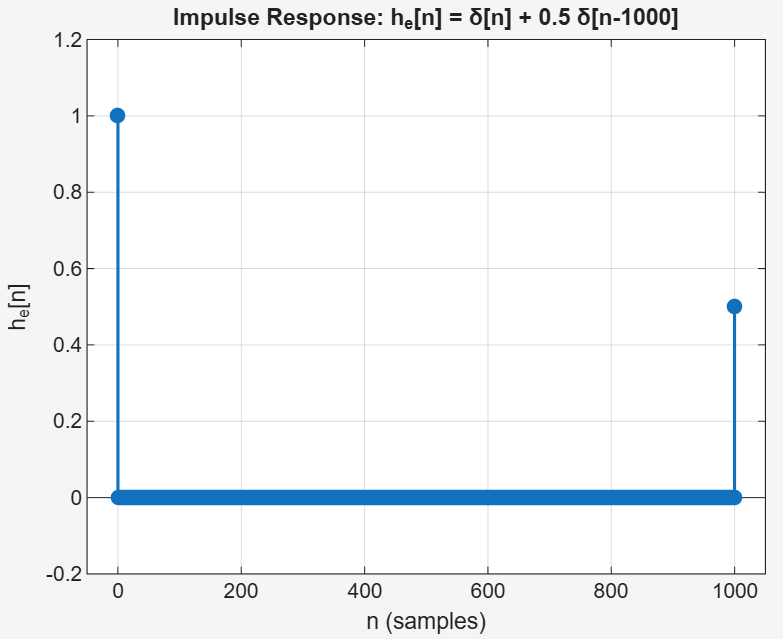
\includegraphics[width=0.5\textwidth]{2.3_1.png}
  \caption{Echo system impulse response}
  \label{fig9}
  \end{figure}



The echo system is:
\begin{equation}
y[n] = x[n] + \alpha x[n - N] \tag{1}
\end{equation}

\begin{equation}
z[n] + \alpha z[n - N] = y[n] \tag{2}
\end{equation}

Substituting (1) into (2):
\begin{equation}
z[n] + \alpha z[n - N] = x[n] + \alpha x[n - N]
\end{equation}

If we propose \(z[n] = x[n]\) as a solution, then:
\begin{itemize}
    \item Left-hand side: \(x[n] + \alpha x[n - N]\)
    \item Right-hand side: \(x[n] + \alpha x[n - N]\)
\end{itemize}

Since both sides are equal, \(z[n] = x[n]\) is a valid solution.

\boxed{\text{Therefore, the inverse system described by } z[n] + \alpha z[n - N] = y[n] \text{ successfully removes the echo}.}



\begin{figure}[H]
  \centering
  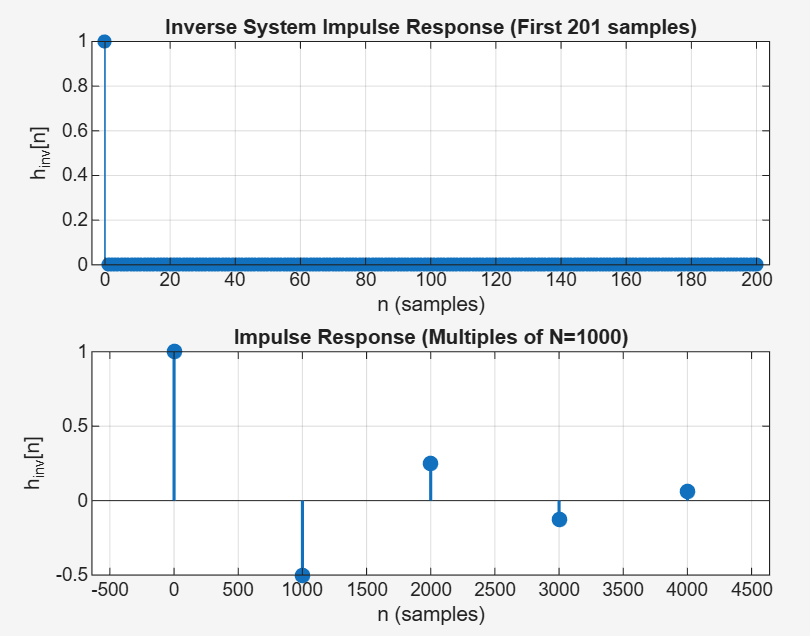
\includegraphics[width=0.5\textwidth]{2.3_2.png}
  \caption{Inverse system}
  \label{fig10}
  
  
\end{figure}


The inverse system is described by:
\[
z[n] + \alpha z[n - N] = y[n]
\]

This is equivalent to:
\[
z[n] = y[n] - \alpha z[n - N]
\]

The system is an IIR (Infinite Impulse Response) filter with coefficients:
\begin{itemize}
    \item \(\mathbf{a} = [1, 0, 0, \ldots, 0, \alpha]\) (length \(N+1\))
    \item \(\mathbf{b} = [1]\)
\end{itemize}

The impulse response \(h_{\text{inv}}[n]\) is obtained by setting \(y[n] = \delta[n]\):

\begin{align}
h_{\text{inv}}[0] &= 1 \\
h_{\text{inv}}[N] &= -\alpha = -0.5 \\
h_{\text{inv}}[2N] &= \alpha^2 = 0.25 \\
h_{\text{inv}}[3N] &= -\alpha^3 = -0.125 \\
&\vdots
\end{align}

The general pattern is:
\[
\boxed{h_{\text{inv}}[k \cdot N] = (-\alpha)^k, \quad k = 0, 1, 2, \ldots}
\]

All other samples are zero. This is an infinite-duration impulse response that decays exponentially as \(k\) increases (since \(|\alpha| < 1\)).

\begin{figure}[H]
  \centering
  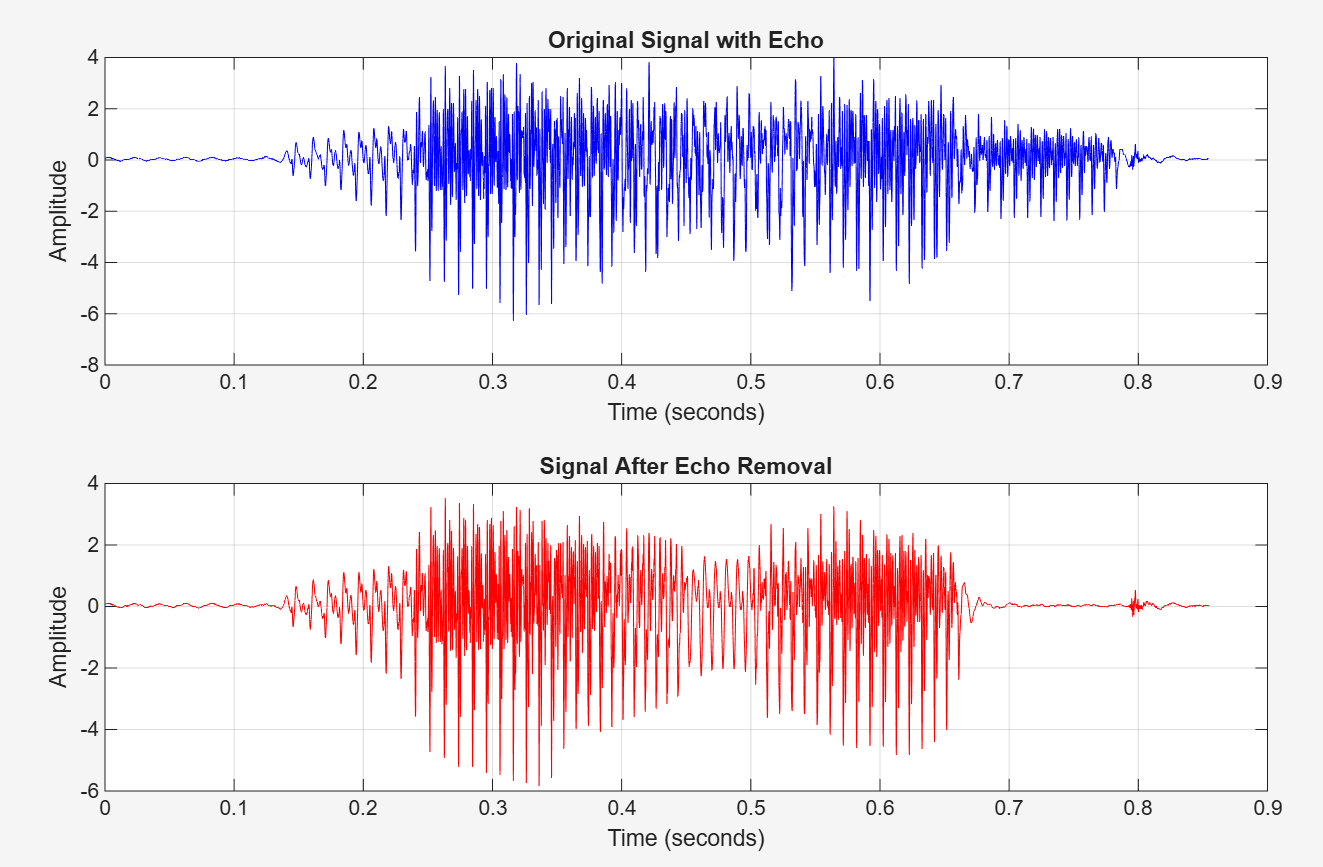
\includegraphics[width=1\textwidth]{2.3_3.png}
  \caption{Inverse system impulse response}
  \label{fig11}

\end{figure}


The echo removal system is implemented using the difference equation:
\[
z[n] + \alpha z[n - N] = y[n]
\]

This can be written as:
\[
z[n] = y[n] - \alpha z[n - N]
\]

\textbf{Implementation:}
\begin{itemize}
    \item Input: \(y[n]\) (speech signal with echo)
    \item Output: \(z[n]\) (speech signal with echo removed)
    \item Parameters: \(N = 1000\), \(\alpha = 0.5\)
\end{itemize}

\textbf{Results:}
\begin{itemize}
    \item The original signal \(y[n]\) contains the phrase "line up" with a noticeable echo.
    \item After processing through the inverse system, the echo is effectively removed.
    \item The output \(z[n]\) sounds like the original uncorrupted speech.
    \item The echo cancellation is successful because the inverse system satisfies \(z[n] = x[n]\).
\end{itemize}



\subsection*{Conclusion}

The echo cancellation system is an inverse filtering approach that recovers the original speech signal from its echo-corrupted version. The key insight is that the echo system is a simple FIR filter, and its inverse is an IIR filter that can be implemented recursively. With proper choice of parameters (\(N = 1000\), \(\alpha = 0.5\)), the inverse system effectively removes the echo while preserving the original speech quality.
\end{document}